\documentclass[11pt]{article}
\usepackage{xcolor}
\usepackage{tikz}
\usepackage{amsmath}
\usepackage{geometry}
\usepackage{algorithm}
\usepackage{algpseudocode}
\usepackage{pgfplots}

\pgfplotsset{width=12cm,compat=1.9}
\geometry{a4paper,scale=0.8}

\definecolor{color1}{RGB}{79, 17, 103} % Blue color
\definecolor{color2}{RGB}{0, 0, 189} % Red color
\definecolor{color3}{RGB}{45, 86, 140} % Green color

\begin{document}

\definecolor{viridis1}{RGB}{68,1,84}
\definecolor{viridis2}{RGB}{58,82,139}
\definecolor{viridis3}{RGB}{32,144,140}
\definecolor{viridis4}{RGB}{94,201,98}
\definecolor{viridis5}{RGB}{253,231,37}

\begin{tikzpicture}
  \draw[step=1cm,black,thick] (0,0) grid (5,5);
  \fill[lightgray] (1, 1) rectangle (2, 2);
  \fill[lightgray] (2, 1) rectangle (3, 2);
  \fill[lightgray] (3, 1) rectangle (4, 2);
  \fill[lightgray] (2, 2) rectangle (3, 3);


  \fill[viridis2] (4, 4) rectangle (5, 5);
  \fill[viridis3] (0, 3) rectangle (1, 4);
  \fill[viridis4] (3, 2) rectangle (4, 3);
  \fill[viridis5] (3, 0) rectangle (4, 1); 

\end{tikzpicture}

% version 1

\begin{algorithm}
    \caption{Weed Clearance Simulation}
    \begin{algorithmic}[1]
    
    \Require $M, n, k_{\text{att}}, k_{\text{rep}}, d_0$
    \Ensure $\max(runtime_i)$ for $i=1 \text{ to } n$
    
    \State $Grid \leftarrow 2D\ Gaussian(M)$
    \State $Agents \leftarrow \{\text{random positions}\}^n$
    
    \While{$|\text{Covered}| < M^2$}
        \For{$a \in Agents$}
            \State $F_{\text{att}}(a) \leftarrow \sum -\frac{k_{\text{att}}}{(1 + d_{ij}^2)^2} \vec{d}_{ij},\ \forall\ \text{cells}$
            \State $F_{\text{rep}}(a) \leftarrow \sum \frac{k_{\text{rep}} (1/d_{ij} - 1/d_0)^3}{d_{ij}^2} \vec{d}_{ij},\ \forall\ \text{covered cells}$
            \State $U(a) \leftarrow \max \left(\frac{1}{\pi} \frac{1}{\gamma  + \theta_{ij}^2}\right),\ \forall\ \text{neighbors}$
            \If{$U(a) > U_{\text{best}}$}
                \State Move $a$ to best cell, update covered
            \EndIf
        \EndFor
    \EndWhile
    
    \State $runtime_i \leftarrow \text{Compute runtime for each } a_i$
    \State \Return $\max(runtime_i)$
    
    \end{algorithmic}
  \end{algorithm}

% version 2

  \begin{algorithm}
    \caption{Weeding Simulation with Strategic Cell Selection}
    \begin{algorithmic}[1]
    
    \State \textbf{Initialize:} Grid $G$ with size $M \times M$, $N$ patches with uniform distribution, $n$ agents with random positions, parameters $k_{\text{att}}$, $k_{\text{rep}}$, $d_0$ and $\gamma$.

    
    \Function{MoveAgent}{$\mathbf{a}, G$}:
        \State Best utility $U_{\text{best}} \gets -\infty$, best move $\mathbf{m} \gets \text{None}$
        \For{each neighbor $\mathbf{n}$ of $\mathbf{a}$}:
            \State Compute total force $\mathbf{F}=\mathbf{F}_{\text{att}}+\mathbf{F}_{\text{rep}}$
            \State $\theta \gets \arctan2(\mathbf{F}[1], \mathbf{F}[0])$
            \State $U \gets C(\theta, \gamma)$, where $\theta$ is mapped to a Cauchy distribution with MAD $\gamma$
            \If{$U > U_{\text{best}}$}:
                \State $U_{\text{best}} \gets U$, $\mathbf{m} \gets \mathbf{n}$
            \EndIf
        \EndFor
        \State \Return $\mathbf{m}$
    \EndFunction
    
    \While{not all cells in $G$ are covered}:
        \For{each agent $\mathbf{a}$}:
            \State Mark cells within vision $\mathbf{m}$ as covered
            \State $\mathbf{m} \gets$ \Call{MoveAgent}{$\mathbf{a}, G$}
            \If{$\mathbf{m} \neq \text{None}$}:
                \State Update $\mathbf{a}$ position to $\mathbf{m}$, mark $\mathbf{m}$ as covered
            \EndIf
        \EndFor
    \EndWhile
    
    \State \textbf{Output:} Maximum runtime among all agents
    
    \end{algorithmic}
    \end{algorithm}

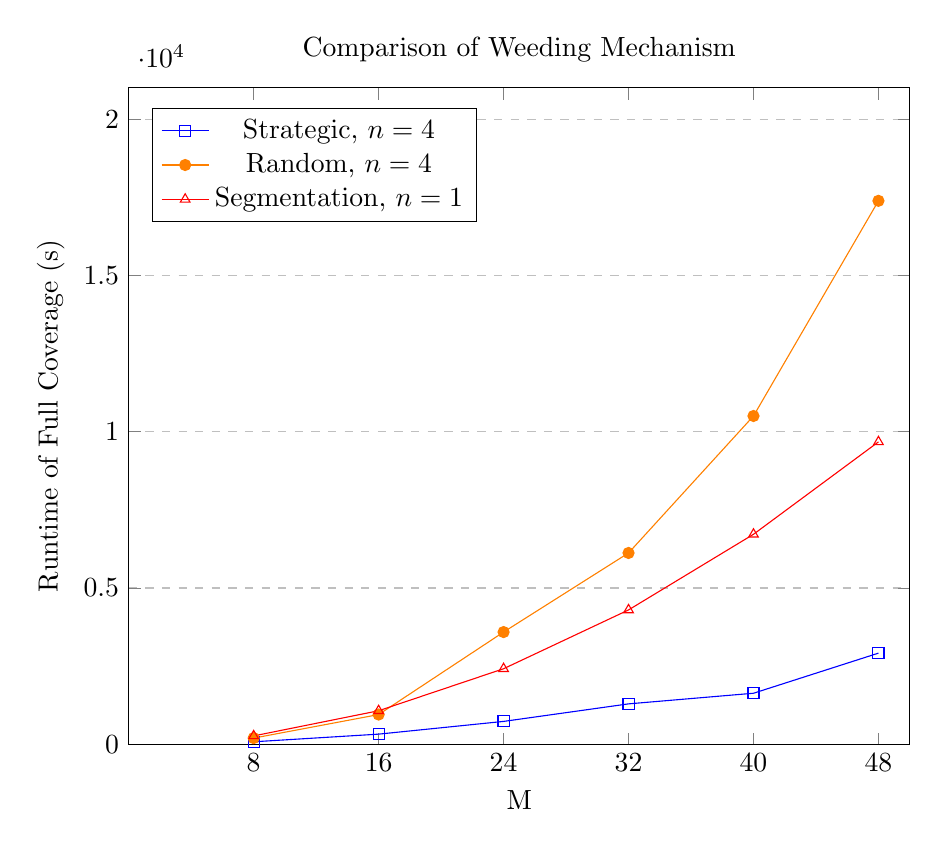
\begin{tikzpicture}
\begin{axis}[
    width=11.5cm,
    title={Comparison of Weeding Mechanism},
    xlabel={M},
    ylabel={Runtime of Full Coverage (s)},
    xmin=0, xmax=50,
    ymin=0, ymax=21000,
    xtick={8,16,24,32,40,48},
    ytick={0,5000,10000,15000,20000},
    legend pos=north west,
    ymajorgrids=true,
    grid style=dashed,
]

\addplot[
    color=blue,
    mark=square,
    ]
    coordinates {
    (8,82)(16,327)(24,734)(32,1295)(40,1635)(48,2918)
    };
    \addlegendentry{Strategic, $n=4$}
    
\addplot[
    color=orange,
    mark=*,
    ]
    coordinates {
    (8,200)(16,953)(24,3592)(32,6122)(40,10504)(48,17387)
    };
    \addlegendentry{Random, $n=4$}
    
\addplot[
    color=red,
    mark=triangle,
    ]
    coordinates {
    (8,270)(16,1075)(24,2419)(32,4300)(40,6720)(48,9676)
    };
    \addlegendentry{Segmentation, $n=1$}
    
\end{axis}
\end{tikzpicture}


% Plot for Table 2: The Effect of Agents in a Field
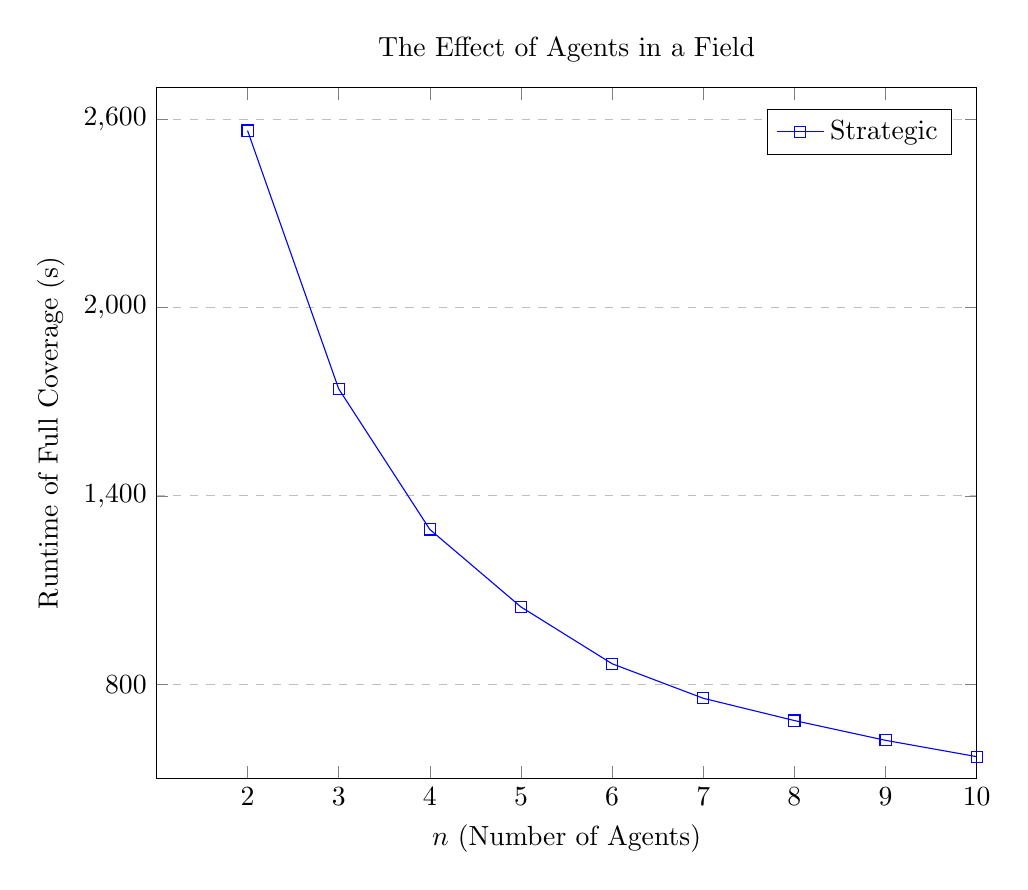
\begin{tikzpicture}
    \begin{axis}[
        title={The Effect of Agents in a Field},
        xlabel={$n$ (Number of Agents)},
        ylabel={Runtime of Full Coverage (s)},
        xmin=1, xmax=10,
        ymin=500, ymax=2700,
        xtick=data,
        ytick={800, 1400, 2000, 2600},
        legend pos=north east,
        ymajorgrids=true,
        grid style=dashed,
    ]
    
    \addplot[
        color=blue,
        mark=square,
        ]
        coordinates {
        (2,2564)(3,1741)(4,1293)(5,1046)(6,865)(7,755)(8,684)(9,621)(10,569)
        };
        \addlegendentry{Strategic}
    
    \end{axis}
    \end{tikzpicture}

    \begin{figure}[h!]
        \centering
        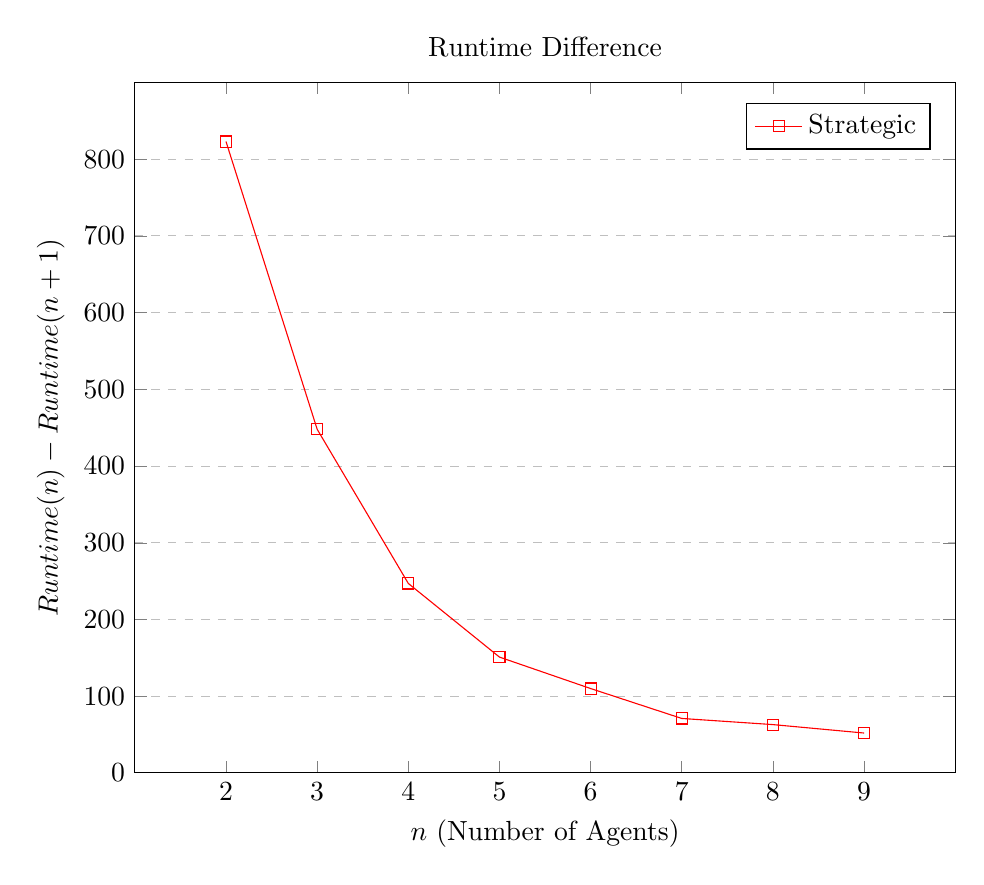
\begin{tikzpicture}
        \begin{axis}[
            title={Runtime Difference},
            xlabel={$n$ (Number of Agents)},
            ylabel={$Runtime(n)-Runtime(n+1)$},
            xmin=1, xmax=10,
            ymin=0, ymax=900,
            xtick={2,3,4,5,6,7,8,9},
            ytick={0,100,200,300,400,500,600,700,800},
            legend pos=north east,
            ymajorgrids=true,
            grid style=dashed,
        ]
        
        \addplot[
            color=red,
            mark=square,
            ]
            coordinates {
            (2,823)(3,448)(4,247)(5,151)(6,110)(7,71)(8,63)(9,52)
            };
            \legend{Strategic}
        
        \end{axis}
        \end{tikzpicture}
        \end{figure}


\begin{figure}[h!]
    \centering
    \begin{minipage}{.5\textwidth}
        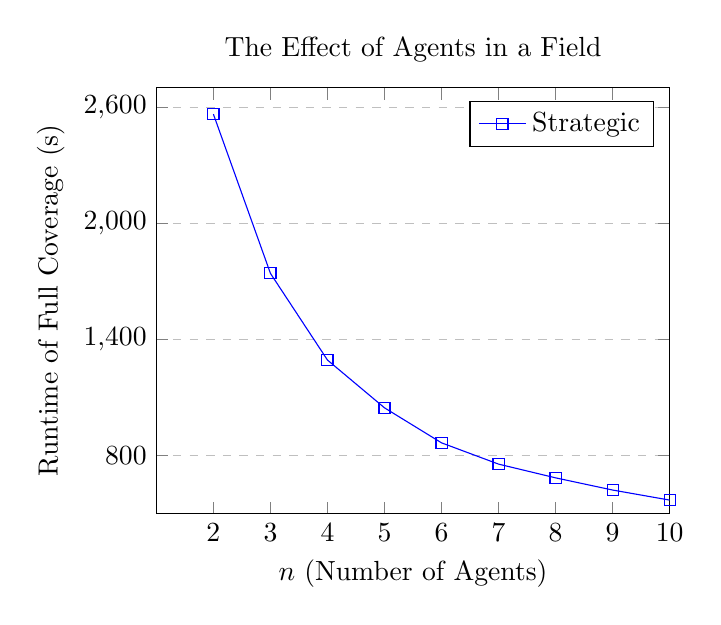
\begin{tikzpicture}
        \begin{axis}[
            width=8.1cm,
            title={The Effect of Agents in a Field},
            xlabel={$n$ (Number of Agents)},
            ylabel={Runtime of Full Coverage (s)},
            xmin=1, xmax=10,
            ymin=500, ymax=2700,
            xtick=data,
            ytick={800, 1400, 2000, 2600},
            legend pos=north east,
            ymajorgrids=true,
            grid style=dashed,
        ]
        
        \addplot[
            color=blue,
            mark=square,
            ]
            coordinates {
            (2,2564)(3,1741)(4,1293)(5,1046)(6,865)(7,755)(8,684)(9,621)(10,569)
            };
            \addlegendentry{Strategic}
        
        \end{axis}
        \end{tikzpicture}
    \end{minipage}%
    \begin{minipage}{.5\textwidth}
        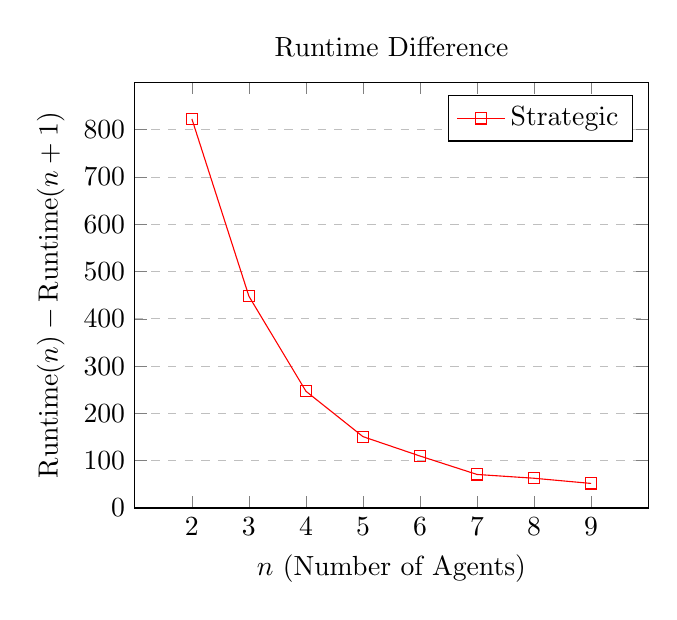
\begin{tikzpicture}
        \begin{axis}[
            width=8.1cm,
            title={Runtime Difference},
            xlabel={$n$ (Number of Agents)},
            ylabel={$\text{Runtime}(n)-\text{Runtime}(n+1)$},
            xmin=1, xmax=10,
            ymin=0, ymax=900,
            xtick={2,3,4,5,6,7,8,9},
            ytick={0,100,200,300,400,500,600,700,800},
            legend pos=north east,
            ymajorgrids=true,
            grid style=dashed,
        ]
        
        \addplot[
            color=red,
            mark=square,
            ]
            coordinates {
            (2,823)(3,448)(4,247)(5,151)(6,110)(7,71)(8,63)(9,52)
            };
            \legend{Strategic}
        
        \end{axis}
        \end{tikzpicture}
    \end{minipage}

\end{figure}


        \begin{figure}[h!]
            \centering
            \begin{minipage}{.5\textwidth}
              \centering
              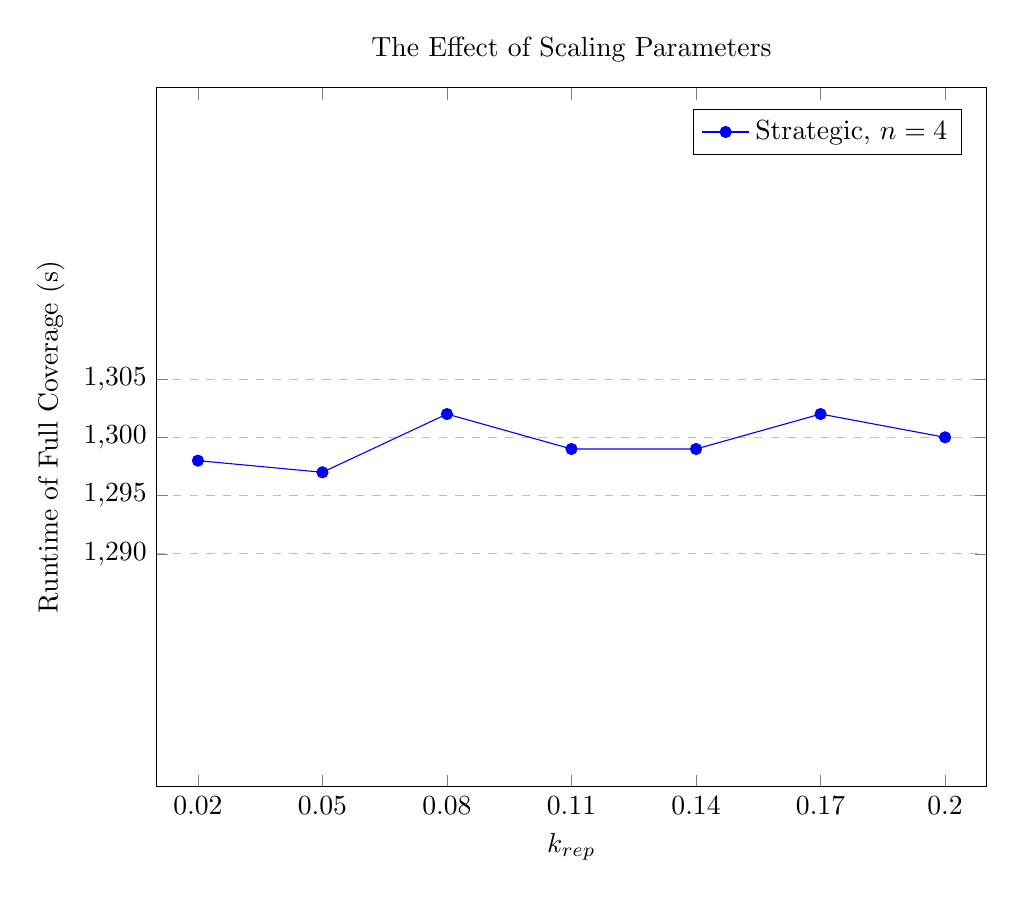
\begin{tikzpicture}
              \begin{axis}[
                  width=\linewidth, % 使图形适应minipage的宽度
                  title={The Effect of Scaling Parameters},
                  xlabel={$k_{rep}$},
                  ylabel={Runtime of Full Coverage (s)},
                  xmin=0.01, xmax=0.21,
                  ymin=1270, ymax=1330,
                  scaled ticks=false,
                  tick label style={/pgf/number format/fixed},
                  xtick={0.02,0.05,0.08,0.11,0.14,0.17,0.20},
                  ytick={1290, 1295, 1300, 1305},
                  legend pos=north east,
                  ymajorgrids=true,
                  grid style=dashed,
              ]
          
              \addplot[
                  color=blue,
                  mark=*,
                  ]
                  coordinates {
                  (0.02,1298)(0.05,1297)(0.08,1302)(0.11,1299)(0.14,1299)(0.17,1302)(0.20,1300)
                  };
                  \addlegendentry{Strategic, $n=4$}
          
              \end{axis}
            \end{tikzpicture}
            \end{minipage}% 注意这里的%号,用来表示注释,也可以防止插入额外的空格
            \begin{minipage}{.5\textwidth}
              \centering
              \begin{tikzpicture}
              \begin{axis}[
                  width=\linewidth, % 使图形适应minipage的宽度
                  title={The Effect of \( d_0 \)},
                  xlabel={\( d_0 \)},
                  xmin=4, xmax=12,
                  ymin=800, ymax=1700,
                  xtick={5,6,7,8,9,10,11},
                  ytick={1000,1100,1200,1300,1400,1500},
                  legend pos=north west,
                  ymajorgrids=true,
                  grid style=dashed,
              ]
          
              \addplot[
                  color=blue,
                  mark=square,
                  ]
                  coordinates {
                  (5,1121)(6,1100)(7,1188)(8,1295)(9,1308)(10,1367)(11,1401)
                  };
                  \addlegendentry{Strategic, $n=4$}
          
              \end{axis}
              \end{tikzpicture}
            \end{minipage}
          \end{figure}
          
    

\end{document}